\documentclass{report}

%\usepackage[latin1]{inputenc}
\usepackage[utf8x]{inputenc}
\usepackage[T1]{fontenc}
\usepackage[french]{babel}
\usepackage[cm]{fullpage}
\usepackage[pdftex]{graphicx}
\usepackage{setspace}
\usepackage{pgfgantt}
\usepackage{comment} 
\usepackage{amsmath}
\frenchbsetup{StandardLists=true}
\usepackage{enumitem}
\usepackage{tikz-uml}
\usepackage{url}
\usepackage{rotating}
\usepackage{hyperref}
\usepackage{appendix}
\usepackage{listings}
\usepackage{xcolor}

\sloppy
\hyphenpenalty 10000000
\definecolor{bargreen}{RGB}{133,193,132}
\definecolor{groupgreen}{RGB}{53,107,52}
\definecolor{darkgreen}{RGB}{35,68,35}
\definecolor{linkred}{RGB}{165,0,33}
\definecolor{comment}{gray}{0.5}

%{Typewriter/teletype family},
\lstdefinestyle{cpp} {
basicstyle=\footnotesize\ttfamily,
language=C++,
captionpos=b,
commentstyle=\color{comment},
deletekeywords={static_cast},
keywordstyle=\color{blue},
morekeywords={LQViewable, GLFWwindow},
numbers=left,
numbersep=10pt,
numberstyle=\tiny\color{comment},
}

\lstdefinestyle{py} {
basicstyle=\footnotesize\ttfamily,
language=Python,
captionpos=b,
commentstyle=\color{comment},
deletekeywords={static_cast},
keywordstyle=\color{blue},
morekeywords={async, await},
numbers=left,
numbersep=10pt,
numberstyle=\tiny\color{comment},
}

\pagestyle{plain}


% TODO : Refaire partie 2.1.1 et 2.1.2 (mieux expliciter framework + décrire ce que l'on fait pour créer une vue)
        % Mettre image des vues de la partie 2.3 dans les annexes
        % Faire les statistique partie 2.4 (Julien)
        % Faire la partie 3 (3.2 + 3.3 = Paul, 3.1 = ?val?)
        % Partie 5
        % Relecture des fautes

\begin{document}

%page de garde
\begin{titlepage}

%logo de la fds, de l'UM et des infos

\includegraphics[scale=0.5]{logoFDS.png}
\hfill

\includegraphics[scale=0.2]{logoInfo.jpg}
\vspace{1cm}

\begin{center}
%au dessus du titre
\textsc{\Large{Rapport de projet T.E.R}} \\
\vspace{1cm}
\textsc{\Large{Projet Informatique HLIN405}} 
\vspace{1.5cm}

%titre
\doublespacing{\textsc{\huge{PunyDuck}}} \\
\vspace{2cm}

\includegraphics[scale=0.5]{logoPunyDuck.jpg}
\vfill
\end{center}

%noms/prenoms + Encadrante
\begin{minipage}[t]{8.5cm}
	\begin{flushleft}
	    \large{\textbf{Etudiants :}}
	    \begin{itemize}[label=]
	        \item \large{Valentin \bsc{FONTAINE}}
	        \item \large{Paul  \bsc{BUNEL}} 
	        \item \large{Esteban \bsc{BARON}}
	        \item \large{Valentin \bsc{PERON}}
	        \item \large{Julien \bsc{LEBARON}}
	    \end{itemize}
		\vspace{0.5cm}
		\large{\textbf{Encadrante :}}
		\large{Anne-Elisabeth \bsc{BAERT}} \\
	\end{flushleft}
\end{minipage}
\hfill
%année universitaire
\begin{minipage}[t]{8cm}
	\begin{flushright} 
		\large{\textbf{Année :} 2020} 
	\end{flushright}
\end{minipage}
\end{titlepage}

%Sommaire
\begin{titlepage}
\renewcommand{\contentsname}{Sommaire}
\setcounter{tocdepth}{1}
\large{\tableofcontents}
\thispagestyle{empty}
\end{titlepage}

%renommer les chapitres en parties
\renewcommand{\chaptername}{Partie}



%Introduction 1/2 pages
\chapter*{Introduction} %Partie présentation
\addcontentsline{toc}{chapter}{Introduction}
Dans le cadre du TER de notre deuxième année à la faculté des sciences de Montpellier nous avons proposé un projet s'intitulant PunyDuck. Le but de ce projet est la réalisation d'une plate-forme de distribution des projets des étudiants du département informatique.\\

Le groupe de développement est composé de cinq personnes, Valentin \textsc{FONTAINE}, Paul \bsc{BUNEL}, Valentin \bsc{PERON}, Julien \bsc{LEBARON} et Esteban \bsc{BARON}. Nous sommes encadré par Mme Anne-Elisabeth \bsc{BAERT}.

\section*{Motivation}

Le TER est un module qui apporte beaucoup aux étudiants en gestion de projet ainsi qu'en programmation. Seulement une fois terminés les projets ne sont pas valorisés et tombent dans l'oubli. Notre solution est de proposer une application permettant à chaque étudiants de déposer leurs projets pour les rendre visibles et téléchargeables par tous.

\section*{Approches}
Notre objectif final étant de produire une application fonctionnelle pouvant être utilisée par tous, nous avions besoin : d'une interface graphique décente, totalement opérationnelle et facilement modulable, ainsi que d'un système de communication efficace entre l'application et la base de données. Nous avons donc décidé de diviser le projet en trois partie : tout d'abord la conception d'un framework permettant la réalisation d'interfaces graphiques, puis la réalisation de l'interface graphique elle-même à partir de ce framework, et enfin la partie réseau permettant à l'application de communiquer avec un serveur distant. Ces trois parties communiquent ensembles part le biais d'une architecture logiciel MVC (Modèle-Vue-Contrôleur).\\
Notre appplication est téléchargeable par tous depuis le site web \url{ https://fvostudio.com/punyduck/}.

\section*{Cahier des charges}
Le but de Punyduck est de proposer aux étudiants en informatique une plateforme de distribution de leurs différents projets. Cette plateforme devait être une application téléchargeable sur un site internet, et connectée à un serveur pour permettre l'échange de projets entre différents clients. \\
Pour l'organisation du projet, nous l'avons tout d'abord divisé en plusieurs étapes : 
\begin{itemize}[label=$-$]
    \item Mise en place d’un serveur qui servira d’intermédiaire entre les utilisateurs et la base de données.
    \item Création d’un framework pour faciliter la réalisation de l’application.
    \item Conception de l’application graphique à l’aide du framework.
    \item Connexion entre l’application graphique et le serveur.
    \item Création d’une base de données pour stocker les comptes des utilisateurs et les
projets.
    \item Mise en service d’un site internet permettant le téléchargement de l’application.
\end{itemize}
\newpage
Ensuite, une fois les différentes parties du projet dégagées, pour bien définir chacune d'entre elles nous avons décidé du cahier des charges suivant :
\begin{description}
%I 
    \item[Le serveur :] Le serveur devra fonctionner de manière asynchrone (nous définiront ce principe dans la prochaine partie). Il pourra héberger de manière sécurisée les données des utilisateurs (nom, mots de passes, ...) et devra être capable de gérer la plupart des erreurs de réseau, comme les coupures de connexion lors d'un téléchargement.
%II
    \item[Le framework :] Le framework définira un ensemble de classes et de fonctions qui serviront de base à la structure d'une nouvelle application. Son utilisation doit être facile avec assez de fonctionnalités déjà disponibles pour pouvoir réduire les appels de fonctions bas niveau. De plus, il devra également permettre la plasticité des interfaces.
%III
    \item[L’application :] Notre application présentera une interface graphique permettant de naviguer facilement entre différents onglets, de communiquer avec le serveur, et de personnaliser un minimum l'apparence : mode clair / sombre, position de certains éléments de la fenêtre, couleur de l’arrière plan.
%IV
    \item[La base de données :] Elle stockera les données relatives aux comptes des utilisateurs ainsi que les projets. Les données confidentielles (mots de passe) seront cryptées.
%V
    \item[Le site :] Il sera constitué d'une unique page permettant de télécharger l'application. Il possèdera un design « responsive~ » et dynamique.
\end{description}

%Quelques définitions ici comme dans l'exemple de rapport ?

%Partie 2 Partie technologies utilisées 1/2 pages
\chapter{Technologies utilisées}
\section{Langages}
Pour la programmation de notre application, nous avons choisis assez naturellement d'utiliser le langage C/C++. En effet, c'est le langage que nous avons le plus étudié à l'université, avec lequel 3 des 5 membres du groupe avaient codé leur projet de Licence 1 CMI, et qui nous offrait un support puissant et efficace pour notre interface graphique. \\
De plus le C++ nous a permis de coder en orienté objet, ce qui était une nécessité pour la création de notre application. En effet, notre programme utilise énormément ce type de programmation : nous développeront ce point plus tard dans la partie 3 sur le développement logiciel. \\

Pour l'interface graphique, nous avons utilisé la bibliothèque OpenGL : une interface regroupant environ 250 fonctions différentes qui peuvent être utilisées pour afficher des scènes tridimensionnelles complexes à partir de simples primitives géométriques. Du fait de son ouverture, de sa souplesse d'utilisation et de sa disponibilité sur toutes les plates-formes, OpenGL est une des bibliothèque graphiques les plus utilisée par la majorité des applications scientifiques, industrielles ou artistiques 3D. \\
L'utilisation de cette bibliothèque (associée à GLFW pour la gestion des fenêtres) était donc un choix assez basique puisqu'elle est très répandue, mais nous avons dû apprendre à l'utiliser : celle-ci est beaucoup plus complexe que les librairies que nous avions utilisées auparavant, comme SFML ou PyGame, de par son bas niveau. \\

Pour gérer la partie réseau de notre application, nous n'avions pas besoin d'utiliser un langage puissant comme le C/C++, nous pouvions donc nous rabattre sur un langage moins performant mais plus facile d'accès.
De ce fait, nous nous sommes dirigés vers le langage python, qui est un langage très simple d'utilisation, pratique pour débuter dans le domaine complexe de la programmation que représente la programmation en réseau. De surcroît il est plutôt efficace pour gérer les entrées sorties, notamment pour la lecture et l'écriture dans des fichiers, qui est une notion centrale dans notre projet.\\

Cependant, le langage Python de base ne permet pas de faire de la programmation en réseau, nous avons donc du choisir une des nombreuses bibliothèques disponibles permettant de faire de la programmation réseau en Python. Après réflexion, nous avons opté pour le module « asyncio » pour deux raisons : premièrement, ce module offrait une interface de programmation en réseau de haut niveau donc plus simple d'utilisation, ce qui nous arrangeait particulièrement étant donné que nous sommes parfaitement novices dans ce domaine ; Deuxièmement, le gros point fort de ce module est le fait qu'il implémente une nouvelle manière de programmer~: la programmation asynchrone. La programmation asynchrone pour les entrées/sorties est une forme de programmation parallèle permettant d'exécuter d'autres parties d'un programme lorsque celui-ci est en attente d'une transmission de donnée, afin de grandement diminuer le temps d'exécution du programme. \\

\section{Outils} %outils utilisés pourquoi ce choix avantages ? postgresql
Pour réaliser notre projet nous avons utilisé des outils différents et spécifiques à chaque tâche. \\

Nous avons utilisé le système de gestion PostgreSQL\footnote{PSQL : \url{https://www.postgresql.org/}} pour gérer la base de données de notre serveur, ce système nous permettant d'utiliser des requêtes SQL en Python et ainsi de mettre en application les connaissances acquises cette année avec le module HLIN304. \\
Pour pouvoir exécuter des requêtes SQL depuis le Python, nous avons employé le module psycopg2\footnote{psycopg2 : \url{https://www.psycopg.org/}} \\

Pour la partie modélisation de l'application nous avons opté pour le Langage de Modélisation Unifié (UML) vu en cours, dans le module HLIN406. \\

Toutes les communications du groupe se sont faites sur le logiciel Discord\footnote{Discord : \url{https://discordapp.com/}}, un logiciel facilitant grandement les communications en groupes avec par exemple le partage d'écran, les groupes vocaux et textuels, le fait de pouvoir partager des morceaux de code directement dans le canal de discussion textuel etc.. \\

Pour ce qui est du partage et des sauvegardes du code, nous avons utilisé Git (un logiciel de gestion de versions décentralisé) via un serveur GitHub\footnote{GitHub : \url{https://github.com/}, notre projet : \url{https://github.com/valfvo/punyduck}} qui nous a permis de garder nos anciennes versions, de ne rien perdre en cours de route, et de pouvoir partager l'avancée du projet avec les autres étudiants du groupes et notre encadrante. \\

Pour ce qui est de l'éditeur de code utilisé, nous nous sommes tous penché sur Visual Studio Code\footnote{VSCode : \url{https://code.visualstudio.com/}} pour sa fiabilité et sa mise en page agréable. De plus, nous avons pu, grâce à ce logiciel, coder à plusieurs en même temps avec sa fonctionnalité de partage en temps réel. \\

Enfin, nous avons utilisé le langage \LaTeX{} via la plateforme Overleaf\footnote{Overleaf : \url{https://www.overleaf.com/}} pour rédiger ce rapport.


%Partie 3 Développement logiciel 5/10 pages
\chapter{Développement logiciel, Conception, Modélisation, Implémentation}
\section{Présentation du développement}
Le développement du projet est séparé en trois parties : 
\begin{itemize}[label=$-$, leftmargin=1.5cm]
    \item le framework de l'interface graphique ;
    \item l'interface graphique utilisant le framework ;
    \item la communication réseau entre le client et le serveur.
\end{itemize}

Le développement de l'application s'est déroulé en plusieurs étapes qui vont être développées points par points.

\subsection{Apprentissage de l'utilisation d'OpenGL}
La première étape fut d'apprendre l'OpenGL, qui fut difficile à comprendre et à utiliser de par son bas niveau comparé aux librairies qu'on a eu l'habitude de voir en L1 et L2. \\
La première partie de l'apprentissage d'OpenGL a été de pouvoir dessiner un triangle d'une certaine couleur. Puis grâce à ce triangle de pouvoir dessiner un rectangle. Ainsi de suite nous avons pu dessiner toutes sortes de formes, tel que les cercles par exemple.
La deuxième partie a été de pouvoir coller des textures sur ces surfaces précédemment créées. Cette partie n'a pas posé réellement de problèmes.
Pour la troisième partie, nous devions pouvoir mettre une surface dans une autre surface, comme dans la figure \ref{exsurface}.
\begin{figure}
    \begin{center}
        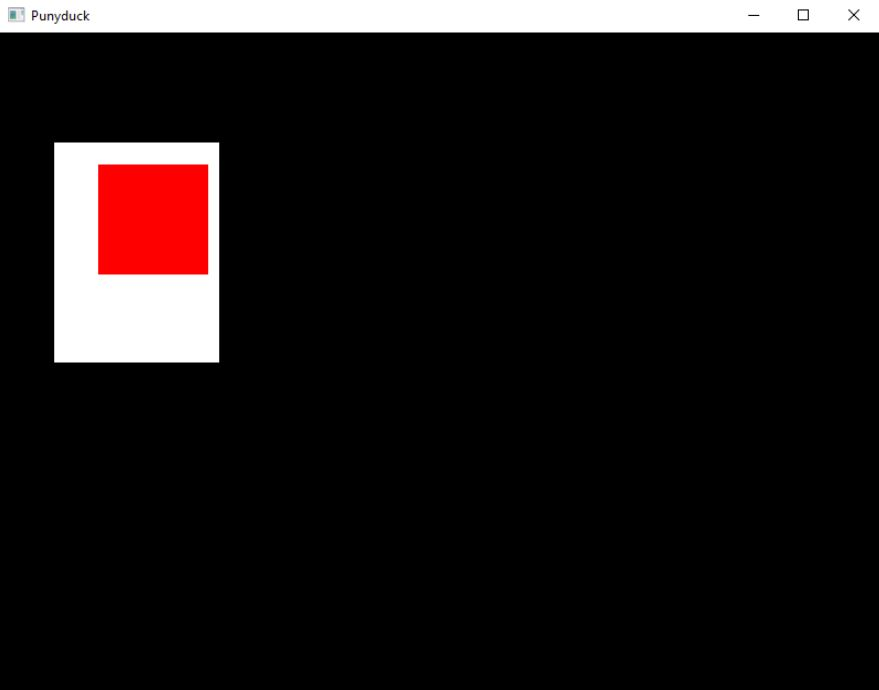
\includegraphics[scale=0.3]{exempleSurface.jpg}
        \caption{Capture d'écran de notre premier essai d'une superposition de surfaces}
        \label{exsurface}
    \end{center}
\end{figure}
Ceci était primordial pour la réalisation de l'application graphique car cette simple tâche a permis la superposition des éléments graphiques de l'application. \\
%plus argumenter sur le texte
La dernière partie était de créer le texte, c'est-à-dire de pouvoir afficher du texte à l'écran. \\

La seconde étape du développement de l'application a été de modéliser en UML les différentes parties de l'application et ses mécanismes. \\
%mieux argumenter ici
Pour commencer, il fallait trouver un système permettant de lier des éléments entre eux afin de pouvoir les superposer, en créer des nouveaux à partir d'anciens, de supprimer un élément et ses sous éléments qui le compose etc..
C'est pour cela que nous avons créé les "Quarks", un système où un élément a un père et n fils (où n appartient à l'intervalle \(\left]0, +\infty\right[\)) et a accès à ses frères. Grâce à ce mécanisme, tous les problèmes cités précédemment ont été résolus. Ce système a donc été la base de toute l'application. \\
Ensuite nous avons créé les différentes classes qui allaient nous servir pour l'implémentation. Comme par exemple : 
%FAIRE LES EXPLICATIONS SUR LES CLASSES COMPLEXES ET SI BESOIN RAJOUTER D'AUTRES CLASSES 
\begin{itemize}[label=$-$]
    \item \verb!LQTexture! qui génère les textures
    \item \verb!LQSurface! pour les surfaces
    \item \verb!LQViewable! 
    \item \verb!LQColor! pour la couleur
    \item \verb!LQNumber! 
    \item \verb!LQText! pour le texte
    \item \verb!LQButton! pour les boutons 
\end{itemize}

%plus argumenter ici
La troisième étape fut la phase d'implémentation. D'une part nous nous sommes occupés des classes en rapport avec d'OpenGL tels que \verb!LQShader!, \verb!LQTexture! et \verb!LQSurface!.
Par la suite nous avons codé les différentes classes en suivant l'UML précédemment réalisé.

\subsection{Création de l'interface graphique}
L'interface graphique a été créée en plusieurs temps. Dans un premier temps il a fallu trouver une représentation graphique validée par tous les membres du groupe. Pour cela, nous avons fait la liste des différentes pages qui seraient dans l'application :
%Je crois que vous avez pas fait les autres pages ? si oui rajoutez-les.
\begin{description}
    \item[Connexion :] une page permettant de s'inscrire et de se connecter à son compte ;
    \item[Projet :] une page affichant tous les projets stockés sur le serveur, où on peut également les télécharger ;
    \item[Dépôt :] une page pour pouvoir déposer ses projets sur l'application.
\end{description}
Puis nous les avons dessinés sur papier une par une, pour que chaque membre du groupe ait une vision très précise de l'aspect visuel de l'application.
Enfin, pour l'implémentation des pages nous avons utilisé le framework créé dans ce but. Il a fallu créer les différents composants de la page pour au final les assembler et former la page souhaitée (une page correspondant à une vue dans notre architecture MVC). \\
Grâce au framework, on a pu lier toutes les pages (vues) entres elles et permettre ainsi la navigation entre les différentes pages de l'application.
Par exemple pour la page "Projet", il a fallut créer cette suite d'éléments qui la composent :
\begin{itemize}[label=$-$]
    \item Une liste de bouton permettant de choisir comment trier les projets ("mieux notés", "plus récents"...)\footnote{\label{note}Cette fonctionnalité n'est pas encore implémentée, c'est donc pour l'instant une simple image}
    \item Une barre de recherche pour accéder à un projet en écrivant son nom
    \item Des boutons qui permettent de trier les projets sous forme de liste ou sous forme de mozaique avec les images des projets\textsuperscript{\ref{note}}
    \item Les projets composés d'un nom, d'un "tag" (jeu, algorithme, application...) et d'une image
\end{itemize}
Une fois créés, nous avons du les assembler pour former la page. Pour cela, la classe \verb!LQTreeCreator! du framework nous a grandement facilité la déclaration des composant et permis une meilleure structure pour la création des pages. C'est une structure d'arbre, chaque composant est un "Quark" qui a une référence sur son père, son précédent frère (\verb!prevSibling!) et sur son prochain (\verb!nextSibling!). 
De plus, on peut accéder à la position des composants avec des méthodes spécifiquement créées telles que \verb!top()!, \verb!right()!, \verb!bottom()!, \verb!left()!. Ainsi nous avons pu placer et créer des composants en fonction de leur père ou des composants précédent ou suivant. \\
Lors de la création des pages avec les composants, nous devions avoir accès au père et aux frères et aux fils. Pour cela les méthodes \verb!sub()! et \verb!super()! ont été créés. La méthode \verb!sub()! permet d'accéder au fils de ce composant, amenant donc la possibilité de créer de nouveaux éléments à partir d'anciens déjà créés.
Une fois le composant souhaité créé, nous pouvons vouloir revenir sur le composant père qui se trouve le plus souvent être la vue en elle-même. Pour cela, on fait appel à la méthode super().\\
Cette structure doit nous faire penser à une structure d'arbre où l'on peut fixer des branches (composant) sur la racine ou sur la branche où l'on se situe.c'est-à-dire créer des branches à partir d'autres branches existantes et fixer cette nouvelle branche à un objet (soit la racine, soit la branche sur laquelle on se situe). 

\subsection{Communication réseau et base de données}
\subsubsection{Réalisation d'un client et d'un serveur}
La partie réseau de notre application s'est faite à part : en effet, elle utilisait un langage différent du reste (le Python) et devait s'exécuter dans un thread secondaire. Cette partie a donc commencé par l'apprentissage de la programmation en réseau via le module asyncio de Python. Ce module étant relativement simple d'utilisation, cette partie n'a pas posé beaucoup de problèmes. \\
Une fois que les bases étaient maîtrisées, nous avons dû créer deux programmes communiquants : un client et un serveur. Le rôle du client était de transmettre les requêtes de l'application au serveur, qui lui devait les analyser, et envoyer une réponse adaptée au client, qui la transmettait à nouveau à l'application. Les requêtes que le serveur devait être capable de gérer étaient peu nombreuses : transfert de projet dans un sens ou dans l'autre (client vers serveur ou serveur vers client) avec ajout dans la base de données, inscription, connexion, et demande de données à la base de données. Ainsi, nous avons opté pour une solution extrêmement simple : pour chacune de ces cinq requêtes, nous associons un numéro (de 1 à 5), que nous insérons au début de la chaîne-requête au moment de sa création dans le C++. Une fois la chaîne envoyée au client python, celui-ci lit le premier octet (donc le numéro de la requête) et exécute la fonction associée. Dans le même temps, il envoie la chaîne au serveur qui fait exactement la même chose. Ainsi, chaque partie de notre système client-serveur sait ce qu'elle doit faire en fonction du besoin de l'application.

\subsubsection{Interface Python/C++}
Une fois le client et le serveur finis et leur fonctionnalités implémentées, nous devions faire communiquer le client avec l'application C++ afin qu'ils puissent se transmettre des informations. Pour cela, nous avons créé en C++ un module Python basique nommé « gateway » utilisant une classe \verb!ClientGateway!. Cette classe contient deux attributs : deux \verb!std::queue! de tableau de charactères, l'une stockant les requêtes à envoyer au serveur, l'autre stockant les réponses (\verb!m_requests! et \verb!m_responses!).\\
Ainsi le module possède deux fonctions : \verb!poll_request! qui retourne le premier élément de \verb!m_requests!, et \verb!transmit_response! qui remplit \verb!m_responses! avec la chaîne passée en paramètre. Le client peut donc communiquer avec l'application de la manière suivante : à chaque tour de boucle, il appelle \verb!poll_request! pour voir s'il a reçu une action à exécuter, puis en cas de réponse du serveur, il transmet les informations nécessaire grâce à \verb!transmit_response!. De la même manière, lorsque l'application veut communiquer avec le client, elle remplit \verb!m_requests! ou regarde le contenu de \verb!m_responses!.\\
Enfin, étant donné que l'application n'a pas accès directement à \verb!m_requests! et \verb!m_responses! puisque que le module s'exécute dans un second thread, nous déclarons une instance de \verb!ClientGateway! dans le contrôleur, puis nous exécutons dans le second thread la fonction de la classe qui lance le programme Python du client. Cette opération nous donne donc accès aux attributs de la \verb!ClientGateway! du second thread directement depuis le contrôleur, dans le premier thread.

\section{Modélisation}

\begin{center}
\begin{tikzpicture}
\umlclass[x=-1,y=-10, fill=gray!5]{LQSurface}{
    -- m\_VBO : GLuint\\
    -- m\_VAO : GLuint\\ 
    -- m\_FBO : GLuint\\
    -- m\_shader : LQShader\\ 
    -- m\_x : LQNumber\\
    -- m\_y : LQNumber\\ 
    -- m\_width : LQNumber\\ 
    -- m\_height : LQNumber\\ 
    %les trois du bas font tout planter peux importe où tu les mets
    %-- m\_clearColor : LQColor\\
    %\umlstatic{-- s\_vertices[54] : GLfloat}\\
    %\umlstatic{-- s\_default\_shader : LQShader}
    }{
    + blit(LQTexture texture, GLfloat x, GLfloat y, GLuint VAO) : void\\
    + fill(GLfloat r, GLfloat g, GLfloat b, GLfloat a=1.0f) : void\\
    + blit(const LQSurface surface) : void\\
    + fill(LQColor color) : void\\
    + move(GLfloat x, GLfloat y) : void\\
    + move(glm::vec2 distance) : void\\
    + moveX(GLfloat x) : void\\
    + moveY(GLfloat y) : void\\
    + moveTo(GLfloat x, GLfloat y) : void\\
    + moveTo(glm\::vec2 position) : void\\
    + moveToX(GLfloat x) : void\\
    + moveToY(GLfloat y) : void\\
    }

\umlclass[x=-5, fill=gray!5]{LQuark}{
    -- m\_parent : LQuark \\
    -- m\_prevSibling : LQuark \\
    -- m\_nextSibling : LQuark \\
    -- m\_firstChild : LQuark \\
    -- m\_lastChild : LQuark \\
    %-- m\_childrenCount : LQuark \\
    }{
    + <<create>>LQuark() \\
    + parent() : LQuark \\
    + firstChild() : LQuark \\
    + lastChild() : LQuark \\
    %+ nthChild(LQindex nth) : LQuark \\
    + prevSibling() : LQuark \\
    + nextSibling() : LQuark \\
    %+ nthSibling(LQindex nth) : LQuark \\
    %+ childrenCount() : LQsize \\
    %+ setNextSibling(LQuark nextSibling): void \\
    + appendChild(LQuark child) : LQuark \\
    %+ insertChild(LQindex index, LQuark child) : LQuark \\
    %+ insertChildBefore(LQuark newChild, LQuark child) : LQuark \\
    %+ insertChildAfter(LQuark newChild, LQuark child) : LQuark \\
    %+ detach() : LQuark \\
    + removeChild(LQuark child) : LQuark \\
    %+ removeFirstChild() : LQuark \\
    %+ removeLastChild() : LQuark \\
    %+ removeChildren(LQuark newParent) : LQuark \\
    %+ swapWith(LQuark quark) : LQuark \\
    %+ swapChildren(LQuark first, LQuark second) : LQuark \\
    %+ swapChildren(LQindex first, LQindex second) : LQuark}
}
\umlclass[x=4.5, fill=gray!5]{LQTexture}{
    -- m\_id : GLuint \\
    -- m\_texWidth : GLuint \\
    -- m\_texHeight : GLuint \\
    -- m\_format : GLuint \\
    -- m\_wrapS : GLuint \\
    -- m\_wrapT : GLuint \\
    -- m\_minFilter : GLuint \\
    -- m\_magFilter : GLuint}{
    + <<create>>LQTexture(string path, int width, int height) \\
    + <<create>>LQTexture(LQTexture other) \\
    + <<create>>LQTexture()\\
    -- genTexture(): GLuint \\
    -- resize(GLuint texWidth, GLuint texHeight):LQTexture\\
    + getId(): GLint \\
    + getWidth(): GLint \\
    + getHeight(): GLint \\
    \umlstatic{+ deleteTexture(LQTexture texture): void}
}

%lien entre bloc
\umlaggreg[mult=5, pos=0.8, angle1=40, angle2=50, loopsize=2cm]{LQuark}{LQuark}
\umlinherit[geometry=-|]{LQSurface}{LQuark}
\umlinherit[geometry=|-]{LQSurface}{LQTexture}
\end{tikzpicture}
\end{center}

\begin{center}
\begin{tikzpicture}
\umlclass[fill=gray!5]{LQNumber}{
    -- m\_quark : LQuark\\
    %-- (*m\_invoke)(LQuark*) : void \\ Trouver comment représenter une fonction en attribut UML
    -- m\_value : float \\
    -- m\_kind : Kind\\
    -- m\_expr : LQMathExpr \\
    -- m\_refs : forward\_list<LQNumber*> \\
    \umlstatic{-- s\_old : float}
}{
    + Kind : enum class ({value,length,coords})\\
    + <<create>>LQNumber() \\
    + <<create>>LQNumber(float value) \\
    + <<create>><<create>>LQNumber(LQMathExpr expr) \\
    + <<create>>LQNumber(Kind kind) \\
    + <<create>>LQNumber(LQNumber other) \\
    + linkQuark(TQuark quark) : void \\
    + recalc() : void \\
    + removeRef(LQNumber ref) : void \\
    + i() : float \\
    + f() : float \\
    + float() : operator \\
    \umlstatic{+ old() : float}
    }
\umlclass[y=-9.5, fill=gray!5]{LQMathVar}{
    -- m\_number : LQNumber \\
    -- m\_coeff : float \\
    -- m\_next : LQMathVar
}{
    + <<create>>LQMathVar(LQNumber number, float coeff=1.0f)\\
    + setNext(LQMathVar next) : void \\
    + eval() : float \\
    + parentCoords(LQNumber number) : bool \\
    + compatible(LQNumber number) : bool
}
\umlclass[x=10, y=-10, fill=gray!5]{LQMathExpr}{
    -- addCompatible(LQMathVar first, float coeff=1.0f) : void\\
    -- m\_first : LQMathVar \\
    -- m\_last : LQMathVar \\
    -- m\_constant : float \\
}{
%    + <<create>>LQMathExpr()\\
    + <<create>>LQMathExpr(LQNumber number)\\
    + <<create>>LQMathExpr(LQMathExpr other)\\
    + eval() : float \\
    + reset() : void \\
    \umlvirt{+ operator=(float constant) : LQMathExpr <<operator>>}\\
    \umlvirt{+ operator=(LQMathExpr expr) : LQMathExpr <<operator>>}\\
    \umlvirt{+ operator+=(float constant) : LQMathExpr <<operator>>}\\
    \umlvirt{+ operator-=(float constant) : LQMathExpr <<operator>>}\\
    \umlvirt{+ operator*=(float coeff) : LQMathExpr <<operator>>}\\
    \umlvirt{+ operator/=(float coeff) : LQMathExpr <<operator>>}\\
    \umlvirt{+ operator+(float constant) : LQMathExpr <<operator>>}\\
    \umlvirt{+ operator+(LQMathExpr other) : LQMathExpr <<operator>>}\\
    \umlvirt{+ operator-(float constant) : LQMathExpr <<operator>>}\\
    \umlvirt{+ operator-(LQMathExpr other) : LQMathExpr <<operator>>}\\
    \umlvirt{+ operator*(float coeff) : LQMathExpr <<operator>>}\\
    \umlvirt{+ operator/(float coeff) : LQMathExpr <<operator>>}
    }
    
\umlclass[x=9, y=2.5, fill=gray!5]{LQuark}{...\\}{...\\}
%lien
\umlaggreg[mult=1, pos=0.5, angle1=40, angle2=60, loopsize=2cm]{LQMathVar}{LQMathVar}
\umlaggreg[mult=1, pos=0.8, angle1=40, angle2=50, loopsize=2cm]{LQNumber}{LQNumber}
\umlassoc[geometry=--, mult=2]{LQMathVar}{LQMathExpr}
\umlassoc[geometry=|-]{LQMathExpr}{LQNumber}
\umlassoc[geometry=--]{LQMathVar}{LQNumber}
\umlassoc[geometry=-|]{LQuark}{LQNumber}
\end{tikzpicture}
\end{center}

\begin{center}
\begin{tikzpicture}
\umlclass[fill=gray!5]{LQViewable}{
    -- m\_flex : bool\\ 
    -- m\_hidden : bool
}{
    %+ <<create>>LQViewable();\\
    + <<create>>LQViewable(LQNumber x, LQNumber y,
               LQNumber width, LQNumber height,\\
               GLint color=0x000000, const std::string iconPath="")\\
    %+ <<create>>LQViewable(LQNumber x, LQNumber y, bool flex=true)\\
    %+ hidden() : bool\\ 
    + hide() : void\\
    + unhide() : void\\
    %+ flexible() : bool\\ 
    + displayFlex() : void\\
    %+ displayBlock() : void\\
    + appendChild(LQViewable child) :  LQViewable\\ 
    + drawChildren() : void \\
    + resizeWidthCallback() : void\\
    \umlvirt{+ resizeHeightCallback() : void}
}
\umlclass[x=-3, y=-5, fill=gray!5]{LQSurface}{...}{...}
\umlclass[x=3, y=-5, fill=gray!5]{LQNumber}{...}{...}
\umlassoc[geometry=--, mult=5, align=center]{LQSurface}{LQNumber}
\umlinherit[geometry=-|]{LQViewable}{LQSurface}
\end{tikzpicture}
\end{center}

\section{Fonctionnalités de l'interface}
%Je parle de ce qui devait être fait (j'ai pas mis les notification, ni personnalisation) si quelque chose ne peux être fait ou n'est pas fait d'ici la fin, enlever directement la partie en question.
Lorsque vous lancerez le client Punyduck vous aurez une interface vous acceuillant dans laquelle vous pourrez vous connectez, avec votre identifiant et votre mot de passe, ou vous inscrire (figure \ref{Connexion}). Une fois connecté vous vous trouverez devant l’interface principale, tout les projets sur PunyDuck seront alors à votre disposition.

L'interface graphique est composé de plusieurs fenêtres, chacune spécifique. Pour les deux fenêtre principales, on a une barre de navigation contenant des liens pour :
\vspace{0.5cm}
\begin{itemize}
    \item Les "Projets", où l'ensemble des projets mis en ligne seront affichés. 
    \item Le "Dépôt" vas servir à faire une demande de dépôt de projet, afin qu'il soit vérifié avant mise en ligne (pour éviter les dépôt de virus ou autre).
    \item Icônes basique telle que réduire, agrandir et fermer.
\end{itemize}
\vspace{0.5cm}

L'interface des projets permet de naviguer à travers les différents projets mis en ligne sur la plateforme et de les rechercher par leur nom ou tag (via la barre de recherche). Pour télécharger un projet, cela se fait simplement via le bouton à droite du tag du projet comme on peut le voir à la figure \ref{Projets}.\\
%Mettre image en annexe (utiliser \appendix)
Pour la page dépôt (figure \ref{Depot}), pour ceux qui souhaitent déposer leur propre projet sur la plateforme, il suffit de cliquer sur l'onglet "dépôt", glisser et déposer votre projet (le dossier) à l'endroit indiqué, lui attribuer un nom puis un tag et enfin l'envoyer en ayant bien remplis tout les champs demandés.
\\

\newpage
%\section{Format des données et procédure d'utilisation} % dnnées utilisées ou encore convention, décrire certaines procédures de lecture et de validation
\section{Statistique} %nombres de classes/scripts/ lignes de code/ nombre de module
Nous allons maintenant regarder notre projet d’un point de vu des statistiques :\\
Le code du logiciel PunyDuck cumule plus de 5400 lignes de code, dont plus de 4000 concernant uniquement les Frameworks. Ces Frameworks sont aux nombres de 28 et, on le vois sur la figure 2.2, ils représentent les trois quart du projet en termes de ligne . Le serveur plus la base de données cumule eux 441 lignes de code, le client 310, le makefile 48, le view 687. Il y a 12 classes utilisées dans ce projet sans compter les frameworks.\\
Le site web est composé d’un fichier html de 175 lignes de code, d’un fichier css de 702 lignes de code et 7 illustrations.

Nous avons également réalisé un module en python qui a aidé pour la réalisation de l'application.\\
Concernant le github, il y a 140 commits en tout, les premiers datant du 19 janvier et les derniers de mai.
\begin{figure}[h]
    \centering
    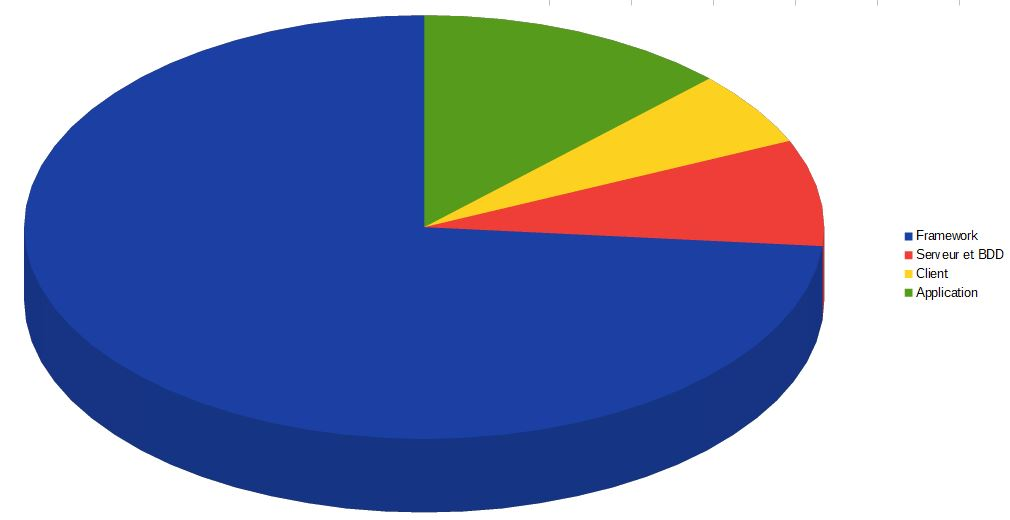
\includegraphics[scale=0.6]{camenbertstatPNDK.JPG}
    \caption{Proportion des lignes de code par rapport au partie du projet}
    \label{fig:my_label}
\end{figure}

%Partie 4 
\chapter{Algorithmes et Structures de Données}
\section{Présentation des principales structures de données}
% Parler de s_eventDispatcher, s_modelObserver, autres ?
\section{Présentation des principaux algorithmes}
Notre application comporte peu d'algorithme poussés, elle est surtout réfléchie au niveau de la communication entre les différentes structures de données qui la composent. Nous allons tout de même présenter ici deux algorithme que nous avons jugés intéressant : la fonction du contrôleur qui s'occupe de savoir, à chaque déplacement du curseur, sur quel élément (\verb!LQViewable!) de la fenêtre il se trouve, et la fonction du serveur qui reçoit les requêtes SQL et renvoie une réponse adapté.
\subsection{Fonction de position du curseur}
La classe \verb!LQAppController! possède un attribut \verb!s_hover_focus! qui est un pointeur vers le dernier \verb!LQViewable! sur lequel s'est positionné le curseur (initialisé sur la fenêtre de l'application lors du lancement du programme).
La méthode \verb!cursor_position_callback! de cette classe est une callback appelée par le module GLFW à chaque déplacement du curseur. Elle prend en paramètre un pointeur vers un objet \verb!GLFWwindow! représentant la fenêtre de l'application, ainsi que les coordonnées absolues du curseur $m_x$ et $m_y$, en nombre réel. Cette méthode calcule sur quel \verb!LQViewable! s'est déplacé le curseur, puis positionne l'attribut \verb!s_hover_focus! du contrôleur sur ce viewable. \\
Etant donné qu'un viewable peut être situé dans un autre élément, et que sa position est relative par rapport à celle de son parent, et non absolue, il nous a fallu trouver une méthode efficace pour retrouver le viewable dans lequel se trouve le curseur. \\

Le fonctionnement de la fonction est donc le suivant\footnote{Tout le long de l'explication de l'algorithme, nous considèrerons les coordonnées en abscisse et en ordonnée comme une seule variable pour plus de simplicité, bien que dans notre programme elles soient séparées en deux variables $x$ et $y$.} : à chaque appel de la fonction, on sauvegarde dans des attributs de la classe \verb!LQAppController! les dernières position absolues et relative (par rapport à \verb!s_hover_focus!) du curseur. Ensuite, nous calculons le déplacement $\Delta$ de la souris :
\[\Delta = m - prevAbs, \text{ avec $prevAbs$ la dernière position absolue du curseur}\]
Ensuite, nous appliquons ce déplacement $\Delta$ sur nos anciennes coordonnées relatives à \verb!s_hover_focus!, afin d'obtenir la nouvelle position relative du curseur par rapport au dernier \verb!LQViewable!. Grâce à cela, nous pouvons définir un booléen important :
\[outCurrent = (prevRel < 0) \vee (prevRel > dim)\]
avec $prevRel$ la position relative du curseur et $dim$ les dimension d'un viewable, ici \verb!s_hover_focus!. \\
Ce booléen nous permet de savoir, selon un viewable, si notre curseur se situe à l'intérieur de celui-ci ou à l'extérieur (en supposant avoir les bonnes coordonnées relative).
Une fois que ceci est fait, il ne nous reste plus qu'à vérifier si notre curseur est toujours dans \verb!s_hover_focus! : si oui, alors on parcours tous ses fils récursivement pour savoir si l'on se trouve dans l'un d'eux ; si non, alors on remonte les parents de \verb!s_hover_focus! jusqu'à trouver celui dans lequel nous sommes, puis nous parcourons également tous ses fils récursivement afin de trouver l'élément le plus précis dans lequel se trouve le curseur. À chaque déplacement dans l'arbre des éléments, nous devons également ajouter ou retirer à $prevRel$ les coordonnées relatives du dernier viewable qu'on a testé, afin que notre booléen $outCurrent$ teste bien avec les bonnes données. \\
Cet algorithme est de complexité $O(n+m)$, avec $n$ la longueur du plus long chemin de l'arbre et $m$ le nombre de fils du noeud avec le plus de fils. L'implantation en C++ de cet algorithme est disponible en annexe \ref{cpc}

\subsection{Fonction de gestion des requêtes SQL}
Quand le serveur reçoit une requête SQL de la part du client, il doit la traiter avant de l'envoyer à la base de données, puis traiter la réponse avant de la renvoyer au client. Tout ceci se fait dans une fonction, que nous allons décrire ici. \\
Tout d'abord, le but de cette fonction est le suivant : elle reçoit en paramètre une chaîne de caractères contenant une requête SQL, et elle envoie au client un \verb!bytearray! contenant, dans l'ordre :
\begin{enumerate}
    \item la chaîne "dataReceive"
    \item suivie du nom du modèle qui recevra les données (afin que le client sache qu'il a reçu des données et à quel modèle elles sont destinées) ;
    \item le nombre d'items reçus (par exemple, si le modèle à modifier est \verb!Project!, un item correspond à un projet) ;
    \item Le nombre total d'attributs de la base de données, ici toujours égal à 15 ;
    \item le nombre d'attributs différents reçus (zéro s'ils sont tous envoyés) suivi de leur id ;
    \item et enfin, les données binaires récupérées dans la base de données grâce à la requête SQL.
\end{enumerate}
Pour cela, on crée en amont de la fonction un dictionnaire en variable globale, qui associe à chaque nom d'attribut de la base de donnée un id :
\begin{lstlisting}[style=py, caption=serveur.py : dictionnaire idColonne, label=idc]
idColonnes = {
    "idProjet": 0,
    "valide": 2,
    "nom": 3,
    "tag": 4,
    "pDescr": 5,
    "pPathImage": 6,
    "pIdLog": 7,
    "idLog": 8,
    "login": 9,
    "password": 10,
    "email": 11,
    "admin": 12,
    "uPathImage": 13,
    "uDescr": 14
}
\end{lstlisting}

Ensuite, la première étape est de savoir si la requête est de type « \verb!SELECT * FROM ...!~ » ou si elle demande des attributs précis de la base de données, par exemple «~ \verb!SELECT idProjet, nom, tag, login FROM Projet, UserInfo WHERE idLog = pIdLog;! ». \\

Dans le premier cas, la fonction exécute la requête dans la base de données et reçoit un tableau de \verb!tuples! en retour, chaque \verb!tuple! correspondant à une ligne de la base de données. On parcours donc chaque élément de ce tableau bidimensionnel, et en fonction de sa position dans le \verb!tuple!, on agit différemment : en effet, on n'ajoute pas la même chose dans la chaîne finale en fonction de si on reçoit une chaîne de caractère, un entier ou un chemin vers une image. Une fois que tous les éléments sont ajoutés à la chaîne finale, il ne reste plus qu'à ajouter les données manquante au début de la chaîne, comme décrit juste avant ("dataReceive", nom du modèle, nombre d'items, etc.). \\

Dans le deuxième cas, c'est plus complexe : avant d'envoyer la requête à la base de données, il faut remettre les attributs dans le même ordre que dans le dictionnaire \verb!idColonnes! (\ref{idc}) afin que le client puisse lire la réponse dans le bon ordre. \\
Pour cela, nous avons implenté en Python l'algorithme triFusion étudié en cours d'algorithmique HLIN301 et HLIN401. En effet, l'objectif est de reconstruire la requête SQL dans le bon ordre avant de l'envoyer à la base de données : nous isolons donc les attributs de la requête dans un tableau grâce aux expressions régulières, puis on appelle notre fonction \verb!triFusion! sur ce tableau (la fonction est adaptée pour pouvoir trier le tableau de chaîne de caractère par rapport au dictionnaire \verb!idColonnes!). Le tableau d'attributs est donc dans le bon ordre après cette opération, nous n'avons plus qu'à reconstruire la requête à partir de ce tableau et à l'exécuter dans la base de données. \\
Une fois que ceci est fait, le reste est essentiellement la même chose que dans le premier cas. \\

Cette fonction s'exécute en temps $O(nm)$ avec $n$ le nombre d'item renvoyé par la base de données et $m$ le nombre d'attributs pour chaque item. Le code Python de cette fonction est disponible en annexe \ref{sql}

%.Partie 5 1/2 pages
\chapter{Gestion du Projet}
\section{Organisation et planification}
Durant le développement de Punyduck, dès son début, nous avons décidé d'avancer le projet après les repas du midi,
ou dès que l'occasion se présentait. Étant toujours ensemble la plupart du temps, c'était donc de manière quotidienne que se faisait l'avancée du projet. Quand le travail se faisait à distance via la plate-forme "discord", nous faisions en sorte de garder toutes traces de ce qui avait été fait, et de ce qui restait à faire, ainsi que de bien penser à mettre le git à jour pour chaque membres du projet.\\

À chaque fin de mois, nous organisions une entrevue avec notre encadrante Mme Anne-Elisabeth \textsc{Baert} afin de faire le point sur l'avancée du projet et de connaître ses priorités. Cela nous a permis de ne pas dériver et d'arriver jusqu'à l'aboutissement du projet. \\

Le développement du projet à été découpé en trois partie (hors site web et rapport) qui sont : la partie réseau en Python (le serveur/client et la base de données PostgreSQL), la partie framework et l'interface de notre application. Le groupe à été séparé au départ en deux groupes : un pour la partie réseau et l'autre pour la partie framework. La dernière partie a réuni les deux groupes afin de produire la liaison Python/C++ et la mise en place de l'interface graphique grâce au framework. \\

Une fois l'ensemble de l'application finie et fonctionnelle, nous avons mit le serveur en ligne afin que l'on puisse lancer l'application de n'importe où. \\
Également, le site web se faisait en parallèle du projet par un Valentin \textsc{Peron} durant cette phase.\\

\section{Changements majeurs}
L'organisation initiale du projet s'est vue considérablement changée tout au long du projet. En premier lieu, nous avons dû gérer la programmation de l'application avec seulement 3 membres du groupes sur les 5. Les tâches ont donc été au départ répartie de la manière suivante : Valentin \textsc{Fontaine} s'occupait du framework, Esteban \textsc{Baron} des débuts de l'interface graphique utilisant le framework, et Paul \textsc{Bunel} de la partie réseau en Python. \\
Puis, une fois ces parties bien avancées, nous avons commencé à mettre en place l'architecture MVC de notre application. À partir de là, nous n'étions plus que deux à s'occuper du code de l'application : ainsi, Valentin \textsc{Fontaine}, aidé par Paul \textsc{Bunel}, se sont donc occupé de l'implémentation de l'architecture MVC, ainsi que de la majorité de l'interface graphique de l'application. \\
Le diagramme de Gantt final du projet est disponnible à la figure \ref{Gantt}.

\newpage
\begin{rotate}{270}
\begin{comment}
%police du gantt au choix selon préférence
\setganttlinklabel{s-s}{START-TO-START}
\setganttlinklabel{f-s}{FINISH-TO-START}
\setganttlinklabel{f-f}{FINISH-TO-FINISH}
\begin{ganttchart}[
    canvas/.append style={fill=none, draw=black!25, line width=3pt},
    hgrid style/.style={draw=black!5, line width=.75pt},
    vgrid={*1{draw=black!5, line width=.75pt}},
    x unit=0.85cm,
    today label font=\small\bfseries,
    title/.style={draw=none, fill=none},
    title label font=\bfseries\footnotesize,
    title label node/.append style={below=7pt},
    include title in canvas=false,
    %Zone des sous parties d'un groupe
    bar label font=\mdseries\small\color{black!90},
    bar label node/.append style={left=1cm},
    bar/.append style={draw=none, fill=darkgreen!60},
    bar incomplete/.append style={fill=bargreen},
    bar progress label font=\mdseries\footnotesize\color{black!70},
    %tête de groupe (Réseau, framwork)
    group incomplete/.append style={fill=groupgreen!85},
    group/.append style={draw=none, fill=darkgreen},
    group left shift=0,
    group right shift=0,
    group height=0.3,
    group peaks tip position=0,
    group label node/.append style={left=1.5cm},
    group progress label font=\bfseries\small,
    %zone rouge / avancement
    link/.style={-latex, line width=1.5pt, linkred},
    link label font=\scriptsize\bfseries,
    link label node/.append style={below left=-1pt and 0pt}
  ]{1}{15}
  \gantttitle[
    title label node/.append style={below left=7pt and -3pt}
  ]{SEMAINES:\quad1}{1}
  \gantttitlelist{2,...,15}{1} \\
  \ganttgroup{Préliminaire Projet}{1}{1} \\[grid]
  \ganttgroup[name = R]{Partie Réseaux}{2}{10} \\
  \ganttbar[progress=75,name=PR1A]{\textbf{PR 1.1} Activité A}{2}{8} \\
  \ganttbar[progress=67,name=PR1B]{\textbf{PR 1.2} Activité B}{2}{10} \\
  \ganttbar[progress=0 ,name=PR1C]{\textbf{PR 1.4} Activité C}{4}{10} \\[grid]
  \ganttgroup{Partie framework}{2}{10} \\
  \ganttbar[progress=0]{\textbf{PFRA 2.1} Activité D}{2}{5} \\
  \ganttbar[progress=0]{\textbf{PFRA 2.2} Activité E}{3}{5} \\
  \ganttbar[progress=0]{\textbf{PFRA 2.3} Activité F}{4}{5}\\[grid]
  \ganttgroup[name= F]{Partie frontwork}{11}{14} \\
  \ganttbar[progress=0]{\textbf{PFRO 2.1} Activité G}{5}{6} \\
  \ganttbar[progress=0]{\textbf{PFRO 2.2} Activité H}{6}{8} \\
  \ganttbar[progress=0]{\textbf{PFRO 2.3} Activité I}{9}{10}\\[grid]
  \ganttgroup{Partie Rapport}{2}{15}\\[grid]
  \ganttgroup{Partie Site web}{9}{13}
  
  %link entre activitées
  \ganttlink[link type=s-s]{PR1A}{PR1B}
  \ganttlink[link type=f-s]{R}{F}
  \ganttlink[link type=f-f,link label node/.append style=left]{PR1C}{PR1B}
\end{ganttchart}
\end{comment}
%plus qu'à compléter
\setganttlinklabel{s-s}{START-TO-START}
\setganttlinklabel{f-s}{FINISH-TO-START}
\setganttlinklabel{f-f}{FINISH-TO-FINISH}
    \begin{ganttchart}[
        hgrid,
        vgrid={*{6}{draw=none},{dotted}},
        vrule/.style={very thick, red},
        x unit=0.160cm,
        time slot format=isodate,
        time slot unit=day,
        calendar week text = {W\currentweek{}},
        bar height = 0.6,
        bar top shift = 0.2,
        bar label node/.append style={align=left,text width={width("--------------------")}},
        bar incomplete/.append style={fill=cyan},
        progress label text = \relax
        link/.style={-latex, line width=1.5pt, linkred},
        ]{2020-01-25}{2020-05-10}
        \gantttitlecalendar{year, month=name, week} \\
        \ganttbar[bar/.append style={fill=groupgreen}, name=ATF]{Asyncio, transfert de fichier}{2020-01-25}{2020-02-24}\\
        \ganttbar[bar/.append style={fill=groupgreen}, name=SQL]{SQL et base de données}{2020-02-25}{2020-03-20}\\
        \ganttbar[bar/.append style={fill=groupgreen}]{Interface python/C++}{2020-03-18}{2020-04-01}\\
        \ganttbar[bar/.append style={fill=darkgreen!60}]{Event et Callback}{2020-03-29}{2020-04-20}\\
        \ganttbar[bar/.append style={fill=darkgreen!60}]{Interface graphique}{2020-04-26}{2020-05-01}\\
        \ganttbar[bar/.append style={fill=bargreen}]{Task6}{2020-02-01}{2020-02-05}\\
        \ganttbar[bar/.append style={fill=bargreen}]{Task7}{2020-02-01}{2020-02-05}\\
        \ganttbar[bar/.append style={fill=bargreen}]{Task8}{2020-02-01}{2020-02-05}\\
        \ganttbar[bar/.append style={fill=bargreen}]{Task9}{2020-02-01}{2020-02-05}\\
        \ganttbar[bar/.append style={fill=bargreen}]{Task10}{2020-02-01}{2020-02-05}\\
        \ganttbar[bar/.append style={fill=bargreen}]{Task11}{2020-02-01}{2020-02-05}\\
        \ganttbar[bar/.append style={fill=bargreen}]{Task12}{2020-02-01}{2020-02-05}\\
        \ganttbar[bar/.append style={fill=bargreen}]{Task13}{2020-02-01}{2020-02-05}\\
        \ganttbar[bar/.append style={fill=bargreen}, name=SW]{Site Web}{2020-03-28}{2020-04-30}\\
        \ganttbar[bar/.append style={fill=bargreen!50}]{Rapport}{2020-04-15}{2020-05-10}
        \ganttvrule{2020-05-30}{2020-04-30}
        %link
        \ganttlink[link type=f-s]{ATF}{SQL}
    \end{ganttchart}
\end{rotate}
\begin{figure}[b]
    \centering
    \caption{Diagramme de Gantt pour notre projet}
    \label{Gantt}
\end{figure}
%.Partie 6 1 page
\chapter{Bilan et Perspectives} %bilan et Conclusion, parler en onction du cahier des charges, les perspectives futur du projet et l'apport.
Le bilan de cette fin de projet est très positive, en comparant à notre cahier des charges, la quasi totalité des demandes et des objectif a été atteints. Malgré le manque de mains d'oeuvres pour la partie informatique, 3 au lieu de 5, le projet à pu voir le jour avec succès.
Bilan partie réseau
Bilan partie front et framework
Bilan des aides (cours, site, grâce à quoi, etc...)

\vspace{1cm}
\section*{Conclusion}

Conclusion globale, point négatif et positif + terminer par les perspectives du client.

%.Partie 7
\part*{Annexes}
\addcontentsline{toc}{part}{Annexes}

\begin{appendix}
\chapter{Visuels de l'application}
\begin{figure}[!h]
    \centering 
    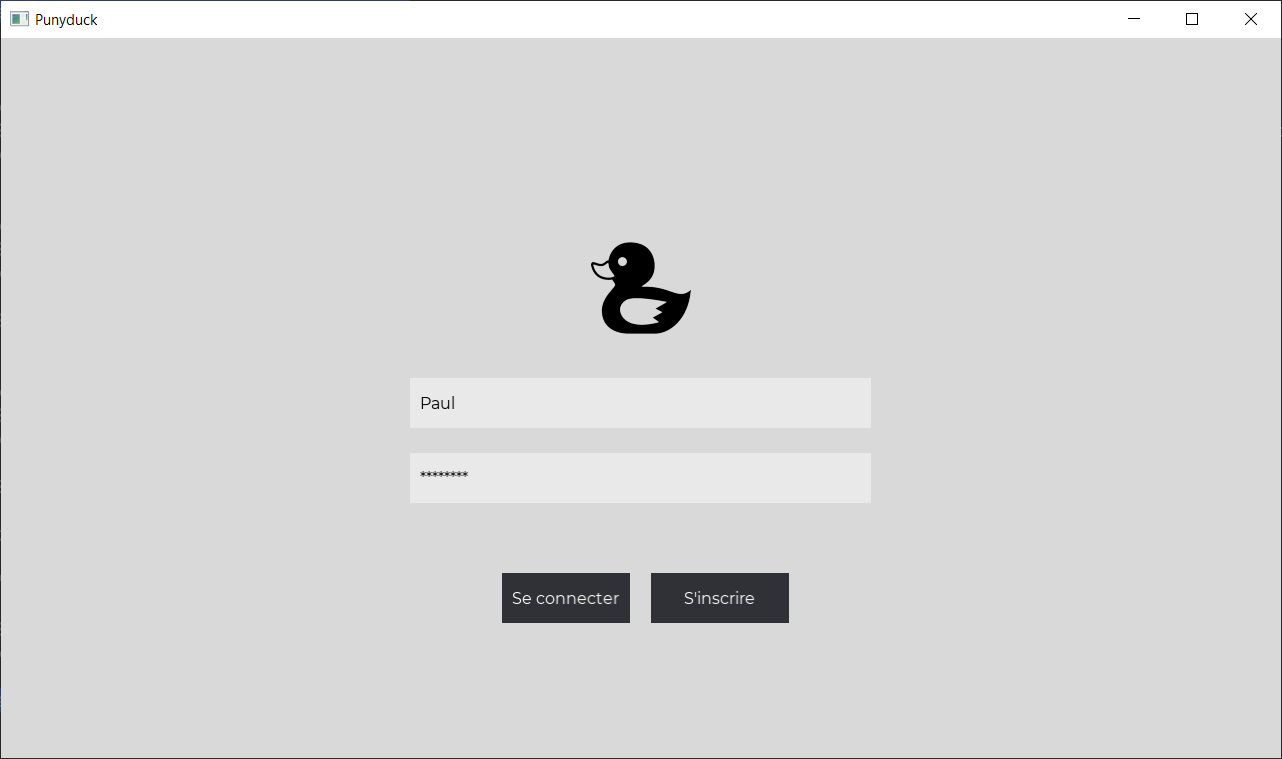
\includegraphics[scale=0.2]{punyduck-img-1.png}
    \caption{Capture d'écran de l'interface de connexion}
    \label{Connexion}
\end{figure}
\begin{figure}
    \centering
    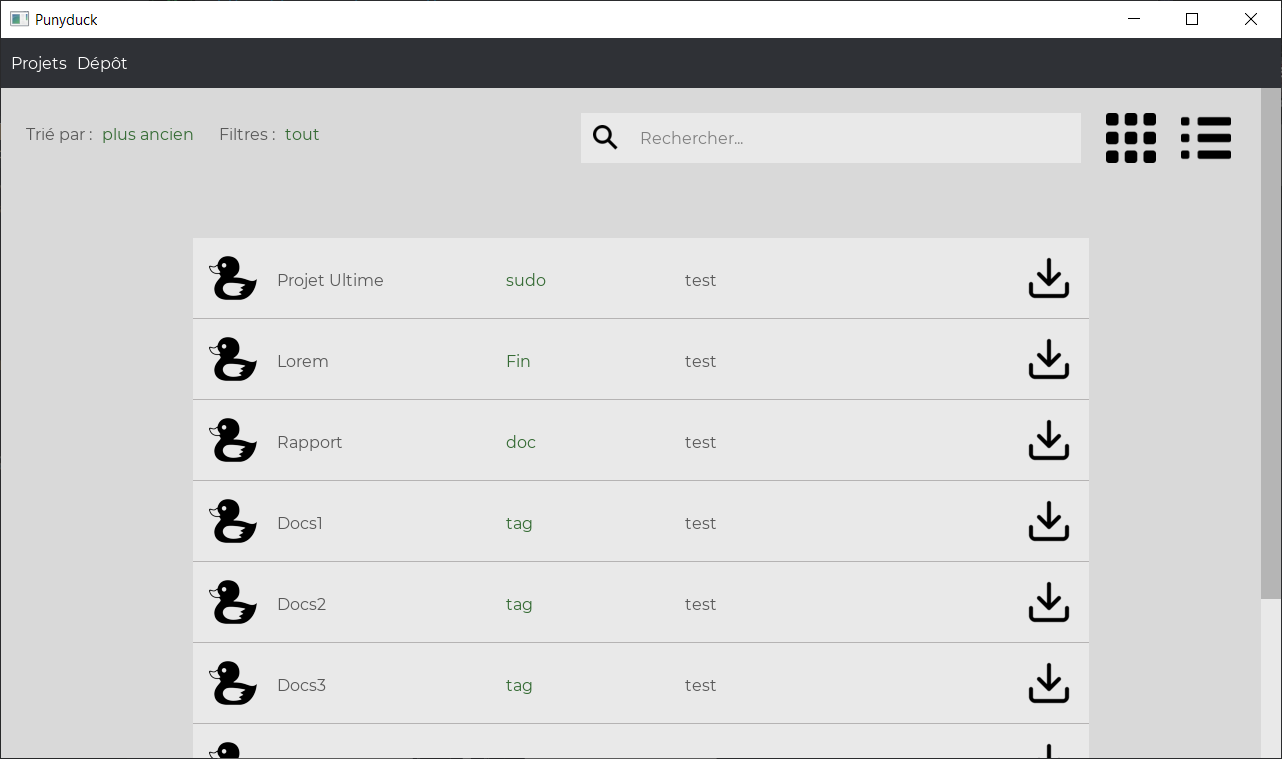
\includegraphics[scale=0.2]{punyduck-img-2.png}
    \caption{Capture d'écran de la page projets}
    \label{Projets}
\end{figure}
\begin{figure}
    \centering
    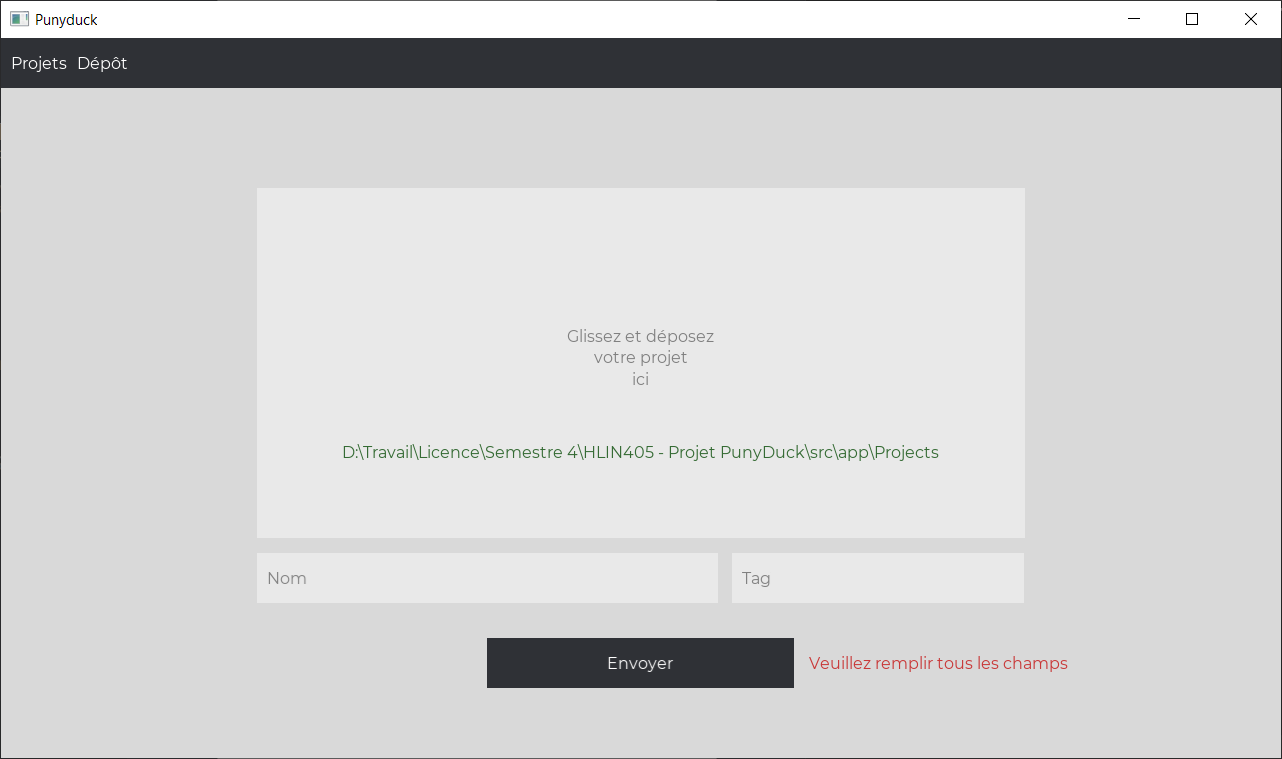
\includegraphics[scale=0.2]{punyduck-img-4.png}
    \caption{Capture d'écran de l'interface de dépôt}
    \label{Depot}
\end{figure}

\chapter{Principaux algorithmes}
\section{Fonction cursor\_position\_callback}
Callback appelée lors d'un déplacement du curseur, calculant le \verb!LQViewable! sur lequel le curseur se positionne.
\begin{lstlisting}[style=cpp, caption=LQAppController::cursor\_position\_callback, label=cpc]
void LQAppController::cursor_position_callback(GLFWwindow* window, double mx, double my) {
    if (my < 50 && prevAbsY >= 50) { // Si la souris est sur la navbar, pas besoin de calculer
        s_hover_focus = static_cast<LQViewable*>(s_window->firstChild());
        prevAbsX = prevRelX = mx;
        prevAbsY = prevRelY = my;
        return;
    }
    float deltaX = mx - prevAbsX;
    float deltaY = my - prevAbsY;
    prevRelX += deltaX;
    prevRelY += deltaY;

    LQViewable* current = s_hover_focus;
    bool outCurrent = prevRelX < 0 || prevRelX > current->widthF() ||
                      prevRelY < 0 || prevRelY > current->heightF();

    while (outCurrent && current != s_window) { // On cherche dans quel parent de s_hover_focus nous sommes
        prevRelX += current->xF();
        prevRelY += current->yF();
        current = static_cast<LQViewable*>(current->parent());
        outCurrent = prevRelX < 0 || prevRelX > current->widthF() ||
                     prevRelY < 0 || prevRelY > current->heightF();
    }

    s_hover_focus = current;
    current = static_cast<LQViewable*>(current->firstChild());
    while (current) { // On recherche un fils correspondant a notre position
        outCurrent =
            prevRelX < current->xF() || prevRelY < current->yF() ||
            prevRelX > current->xF() + current->widthF() ||
            prevRelY > current->yF() + current->heightF();
        if (outCurrent) {
            current = static_cast<LQViewable*>(current->nextSibling());
        }
        else {
            s_hover_focus = current;
            prevRelX -= current->xF();
            prevRelY -= current->yF();
            current = static_cast<LQViewable*>(current->firstChild());
        }
    }

    prevAbsX = mx;
    prevAbsY = my;
}
\end{lstlisting}

\section{Fonction SQL}
Fonction exécutée par le serveur lorsque le client envoie une requête SQL.

\begin{lstlisting}[style=py, caption=serveur.py : SQL, label=sql]
def fusion(T1, T2, T):
    i1 = 0
    i2 = 0
    for i in range(len(T)):
        if i1 >= len(T1):
            T[i] = T2[i2]
            i2 += 1
        elif i2 >= len(T2):
            T[i] = T1[i1]
            i1 += 1
        elif idColonnes[T1[i1]] < idColonnes[T2[i2]]:
            T[i] = T1[i1]
            i1 += 1
        else:
            T[i] = T2[i2]
            i2 += 1

def triFusion(T): # Algorithme triFusion vu en cours HLIN301 et HLIN401
    if len(T) > 1:
        T1 = T[:int(len(T)/2)]
        triFusion(T1)
        T2 = T[int(len(T)/2):]
        triFusion(T2)
        
        fusion(T1, T2, T)

nAttributes = int(15).to_bytes(1, 'big')

async def SQL(writer, query):
    # query = model + requete SQL
    model = re.search(r'(.*)SELECT', query).group(1)
    query = re.search(r'(SELECT.*)', query).group(1)

    infos = b''
    nItems = 0

    if "*" in query: # Si la requete est du type "SELECT * FROM ..."
        cur.execute(query)
        datas = cur.fetchall()

        ordreIndice = int(0).to_bytes(4, 'big')
        if "Projet" in query:
            for data in datas:
                for row in range(len(data)): # On agit differemment en fonction du type de donnees
                    if row == 1 or row == 6:
                        img = Image.open(data[row].replace("\\\\", "\\"))
                        infos += img.width.to_bytes(4, 'big')
                        infos += img.height.to_bytes(4, 'big')
                        infos += GL_RGBA if img.mode == "RGBA" else GL_RGB
                        infos += len(img.tobytes()).to_bytes(4, 'big')
                        infos += img.tobytes()
                    elif row == 0 or row == 7 or row == 2:
                        infos += data[row].to_bytes(4, 'big')
                    else:
                        infos += data[row].encode() + b'\0'
                nItems += 1

        elif "UserInfo" in query:
            for data in datas:
                for row in range(len(data)): # On agit differemment en fonction du type de donnees
                    if row == 5:
                        img = Image.open(data[row])
                        infos += img.width.to_bytes(4, 'big')
                        infos += img.height.to_bytes(4, 'big')
                        infos += GL_RGBA if img.mode == "RGBA" else GL_RGB
                        infos += len(img.tobytes()).to_bytes(4, 'big')
                        infos += img.tobytes()
                    elif row == 0:
                        infos += data[row].to_bytes(4, 'big')
                    else:
                        infos += data[row].encode() + b'\0'
                nItems += 1
    
    else: # Si la requete est du style "SELECT ..., ... FROM ..."
        match = re.search(r'^SELECT (.*) FROM .*;', query)
        if match != None:
            # On remet les attributs dans l'ordre afin de les recevoir correctement, et que le
            # client les recoive dans l'ordre
            rows = match.group(1).split(', ')
            endQuery = re.search(r'(FROM.*)', query).group(1)
            triFusion(rows)
            query = "SELECT "
            for row in rows[:-1]:
                query += row + ", "
            query += rows[-1] + " " + endQuery

            # On sauvegarde l'ordre d'arrivee des attributs de la base de donnees
            ordreIndice = len(rows).to_bytes(4, 'big')
            for row in rows:
                ordreIndice += idColonnes[row].to_bytes(4, 'big')

            cur.execute(query)
            datas = cur.fetchall()

            for data in datas:
                for row in range(len(data)): # On agit differemment en fonction du type de donnees
                    if idColonnes[rows[row]] == 0 or idColonnes[rows[row]] == 2 or idColonnes[rows[row]] == 7 or idColonnes[rows[row]] == 8:
                        infos += data[row].to_bytes(4, 'big')
                    elif idColonnes[rows[row]] == 6 or idColonnes[rows[row]] == 13:
                        fp = open(data[row], 'rb')
                        img = Image.open(fp)
                        infos += img.width.to_bytes(4, 'big')
                        infos += img.height.to_bytes(4, 'big')
                        infos += GL_RGBA if img.mode == "RGBA" else GL_RGB
                        infos += len(img.tobytes()).to_bytes(4, 'big')
                        infos += img.tobytes()
                    else:
                        infos += data[row].encode() + b'\0'
                nItems += 1

        # On construit la chaine a renvoyer au client
        infos = "dataReceive".encode() + b'\0' + model.encode() + b'\0' + \
                nItems.to_bytes(4, 'big') + nAttributes + ordreIndice + infos
        # str + \0 + str + \0 + 4 bytes + 1 byte + (4 bytes + 4 * nbIndice bytes) + n bytes
        
        await send_message(writer, infos)
\end{lstlisting}
\end{appendix}

\end{document}
